\documentclass[a4paper]{article}

\usepackage[fontset=fandol]{ctex}
\usepackage{amsmath, amssymb}
\usepackage{graphicx}
\usepackage[margin=2.3cm]{geometry}
\usepackage[most]{tcolorbox}
\usepackage{etoolbox}
\usepackage{listings}
\usepackage{hyperref}
\usepackage{xurl}
\usepackage{booktabs}
\usepackage{longtable}
\usepackage{tabularx}
\usepackage{array}
\usepackage{subcaption}
\usepackage{float}
\usepackage{enumitem}
\usepackage{tikz}
\usetikzlibrary{arrows.meta, positioning, shapes.geometric, fit}
\IfFileExists{pgfplots.sty}{
    \usepackage{pgfplots}
    \pgfplotsset{compat=1.18}
}{}

\hypersetup{
    colorlinks=true,
    linkcolor=blue!50!black,
    urlcolor=blue!60!black,
    citecolor=blue!50!black
}

\newtcolorbox{findingbox}[1]{
    enhanced,
    colback=green!5!white,
    colframe=green!45!black,
    colbacktitle=green!45!black,
    coltitle=white,
    fonttitle=\bfseries,
    title=#1,
    sharp corners
}

\newtcolorbox{evidencebox}[1]{
    enhanced,
    colback=blue!4!white,
    colframe=blue!65!black,
    colbacktitle=blue!65!black,
    coltitle=white,
    fonttitle=\bfseries,
    title=#1,
    sharp corners
}

\newtcolorbox{riskbox}[1]{
    enhanced,
    colback=red!4!white,
    colframe=red!70!black,
    colbacktitle=red!70!black,
    coltitle=white,
    fonttitle=\bfseries,
    title=#1,
    sharp corners
}

\newtcolorbox{methodbox}[1]{
    enhanced,
    colback=yellow!9!white,
    colframe=yellow!60!black,
    colbacktitle=yellow!60!black,
    coltitle=black,
    fonttitle=\bfseries,
    title=#1,
    sharp corners
}

\lstset{
    language=Python,
    basicstyle=\ttfamily\small,
    keywordstyle=\color{blue},
    stringstyle=\color{red!60!black},
    commentstyle=\color{green!50!black},
    breaklines=true,
    frame=single,
    numbers=left,
    numberstyle=\tiny\color{gray},
    captionpos=b,
    extendedchars=false
}

\newcolumntype{Y}{>{\raggedright\arraybackslash}X}
\setlist[itemize]{leftmargin=1.8em}

\newcommand{\reporttitle}{视频笔记可视化链路深度研究}
\newcommand{\reportsubtitle}{从字幕之后到高质量 PDF：对现有 skill / runtime 的诊断、外部方案扫描与改造路线}
\newcommand{\reportauthors}{Codex}
\newcommand{\reportdate}{2026-03-26}
\newcommand{\researchquestion}{如何优化 video-note skill 与 video-note-pipeline 在“字幕获取之后”的可视化链路，使 agent 更稳定地产出逻辑连贯、图像清晰、来源可追踪的高质量 PDF？}
\newcommand{\reportscope}{聚焦字幕之后的视觉与排版阶段：视频定位、候选帧搜索、裁剪与 OCR、图文规划、PDF 构建、联网增益、评测体系。证据来自本地两个实现、多个历史 case，以及截至 2026-03-26 的公开官方文档与项目资料。}
\newcommand{\reportaudience}{video-note skill / runtime 的维护者，以及需要把视频系统化沉淀为研究型 PDF 的 agent 设计者}
\newcommand{\sourcewindow}{本地仓库状态截至 2026-03-26；外部网页资料访问日期为 2026-03-26}
\newcommand{\reportcoverpath}{figures/current-overview-montage.jpg}

\begin{document}

\begin{titlepage}
\centering
{\Large 深度研究报告\par}
\vspace{1.0cm}
{\huge\bfseries \reporttitle\par}
\vspace{0.5cm}
{\Large \reportsubtitle\par}
\vspace{0.9cm}
{\large \reportauthors\par}
\vspace{0.2cm}
{\large \reportdate\par}
\vspace{1.0cm}
\includegraphics[width=0.84\textwidth,height=0.42\textheight,keepaspectratio]{\reportcoverpath}\par
\vfill
\begin{tcolorbox}[width=0.94\textwidth, colback=black!2!white, colframe=black!60, sharp corners]
\textbf{核心问题}：\researchquestion\par
\textbf{研究范围}：\reportscope\par
\textbf{目标读者}：\reportaudience\par
\textbf{证据窗口}：\sourcewindow\par
\end{tcolorbox}
\end{titlepage}

\tableofcontents
\newpage

\section{执行摘要}

\begin{findingbox}{核心结论}
当前链路的主要瓶颈不是“字幕之后没有任何工具”，而是“字幕之后没有稳定的中间层”。旧 \texttt{video-note-skill} 已经写出了高质量 figure workflow 的原则，但主要依赖执行者手工执行；新的 \texttt{video-note-pipeline} 则把 preflight / transcript / overview / build 结构化了，却还没有把 figure planning、候选帧密集搜索、裁剪、manifest、叙事构建、PDF QA 变成 runtime 能直接产出的确定性步骤。
\end{findingbox}

\begin{itemize}
\item 现有 runtime 在字幕之后真正拥有的能力，主要只有均匀抽样 overview、Pillow montage、基于重复率和熵的粗 mode heuristic，以及 LaTeX 编译包装；这对于“先粗分视频类型”足够，但对“稳定产出高质量 PDF”明显不够。
\item 本地 case 已经给出清晰证据：\texttt{static-outline} 视频需要尽早放弃密集原始截图，转向少量高价值裁剪图与 TikZ；\texttt{board-heavy} 长视频需要 \texttt{candidate -> montage -> crop-first} 的分层策略；\texttt{commentary} 视频里 OCR 大规模失效，应转向“正文主导 + 少量 representative frames + 自制结构图”。
\item 外部项目和官方文档说明，可用方案非常丰富，但应按层接入。P0 阶段并不需要重型 CV 栈，只要把 \texttt{ffmpeg + Pillow + manifest} 产品化，就能获得最大一批收益；P1 再引入 PySceneDetect、PaddleOCR layout / formula、可选的 OCR / layout probes；P2 再考虑 VLM 或学习型 shot boundary。
\item 对 PDF 渲染层的建议不是“马上换掉 LaTeX”，而是“保留 LaTeX、重构输入中间层”。与其直接从 transcript 跳到 \texttt{note.tex}，不如先生成 \texttt{outline.json}、\texttt{claims.json}、\texttt{figure\_plan.json}、\texttt{frame\_manifest.json}、\texttt{render\_context.json}，再渲染 TeX。
\item 联网增强值得做，但不应塞到最后 build 阶段，而应放到 claims 定稿前，并且必须模式化控制：忠实讲义默认关闭或仅补拓展阅读；评论 / 分析 / 证据敏感视频才开启外部事实核验与背景补全。
\end{itemize}

\begin{riskbox}{最重要的工程决策}
如果直接补很多模型和工具，却不先定义 artifact contract，最后只会把人工 figure workflow 变成更复杂的人工 figure workflow。应先固定流程产物，再增加模型能力。
\end{riskbox}

\section{研究范围与方法}

\subsection{研究对象与时间边界}

本报告聚焦于“字幕已经拿到之后”的阶段，即：

\begin{itemize}
\item transcript 如何转成教学单元、章节与论点；
\item 如何从视频中定位候选图、搜索最终帧、做 crop；
\item 如何在 PDF 中把截图、重绘图、表格、正文、provenance 组织成逻辑更连贯的文档；
\item 是否以及如何在这一阶段引入联网检索来增强背景、佐证或纠错。
\end{itemize}

本地实现包括：

\begin{itemize}
\item 旧 skill：\path{/home/fanghaotian/.codex/skills/video-note-skill/skills/bilibili-render-pdf/SKILL.md}
\item 当前 runtime：\path{/home/fanghaotian/Desktop/src/video-note-pipeline}
\item 当前统一 wrapper：\path{/home/fanghaotian/Desktop/src/agent-basic-skill/skills/video-note-render-pdf}
\item 历史 case：\path{/home/fanghaotian/Desktop/src/video_notes}
\end{itemize}

\subsection{方法}

\begin{methodbox}{证据构成}
\begin{itemize}
\item 本地代码与模板：检查 runtime 真实能力边界，以及 skill 当前的写作与 figure 规则。
\item 本地 retrospective 与案例：提取真实运行中的断点、补救动作、稳定有效的经验。
\item 外部官方文档 / 官方仓库：调研 scene detection、slide extraction、OCR / layout、PDF authoring、文档中间表示等主流方案。
\item 综合判断：在“你们现在已有 skill / runtime / case 资产”的约束下，优先选择最小改动、最高 ROI 的升级路线，而不是理论上最强但工程代价过高的方案。
\end{itemize}
\end{methodbox}

\subsection{研究问题拆解}

用户在本轮讨论里提出了五个直觉问题，本报告将逐一回答：

\begin{enumerate}
\item 图片处理工具是否不够，尤其是不方便 crop？
\item 视频处理是否不够好，导致定位关键图片不准？
\item PDF 构建是否还有更好的方式，让逻辑更连贯、动机更清晰？
\item 构建 PDF 时是否应该联网搜索，以获得额外资源和背景？
\item 历史 case 能否被系统化为评测集与流程约束？
\end{enumerate}

\section{当前实现与案例证据}

\subsection{旧 skill 的优点：原则完整，但执行主要靠 agent}

旧 \texttt{bilibili-render-pdf} 在规则层面对 figure handling 的描述其实很强。它明确要求：

\begin{itemize}
\item 以字幕时间窗作为关键帧定位主线；
\item 先高召回搜索候选，再人工下采样；
\item 对渐进式 reveal、白板累积、界面变化要找最终完整可读状态；
\item 必要时 crop；
\item 对难以用截图解释的内容补 TikZ / PGFPlots 或脚本生成图；
\item 记录视频图像的时间区间 provenance。
\end{itemize}

这些规则见 \path{/home/fanghaotian/.codex/skills/video-note-skill/skills/bilibili-render-pdf/SKILL.md} 的 Figure Handling 与 Visualization 段落。问题不在理念，而在于这些步骤还没有被落为 runtime artifact，因此无法稳定复用。

\subsection{新 runtime 的优点：壳已经搭好，但视觉中间层缺失}

当前 \texttt{video-note-pipeline} 的优点，是已经把 preflight、subtitle / transcript 获取、overview、build 这些“壳”结构化了。但字幕之后真正自动化的部分只有四个：

\begin{itemize}
\item \texttt{extract\_overview\_frames}: 对整段视频均匀抽样；
\item \texttt{build\_montage}: 用 Pillow 做缩略图拼版；
\item \texttt{infer\_recommended\_mode}: 用重复率、熵、相邻差分做粗 heuristic；
\item \texttt{build\_note}: 执行 LaTeX 编译与预览导出。
\end{itemize}

这从 \path{/home/fanghaotian/Desktop/src/video-note-pipeline/src/video_note_pipeline/frames/overview.py}、
\path{/home/fanghaotian/Desktop/src/video-note-pipeline/src/video_note_pipeline/commands.py}、
\path{/home/fanghaotian/Desktop/src/video-note-pipeline/src/video_note_pipeline/build/latex.py} 可以直接确认。

\begin{figure}[H]
\centering
\begin{subfigure}[t]{0.48\textwidth}
\centering
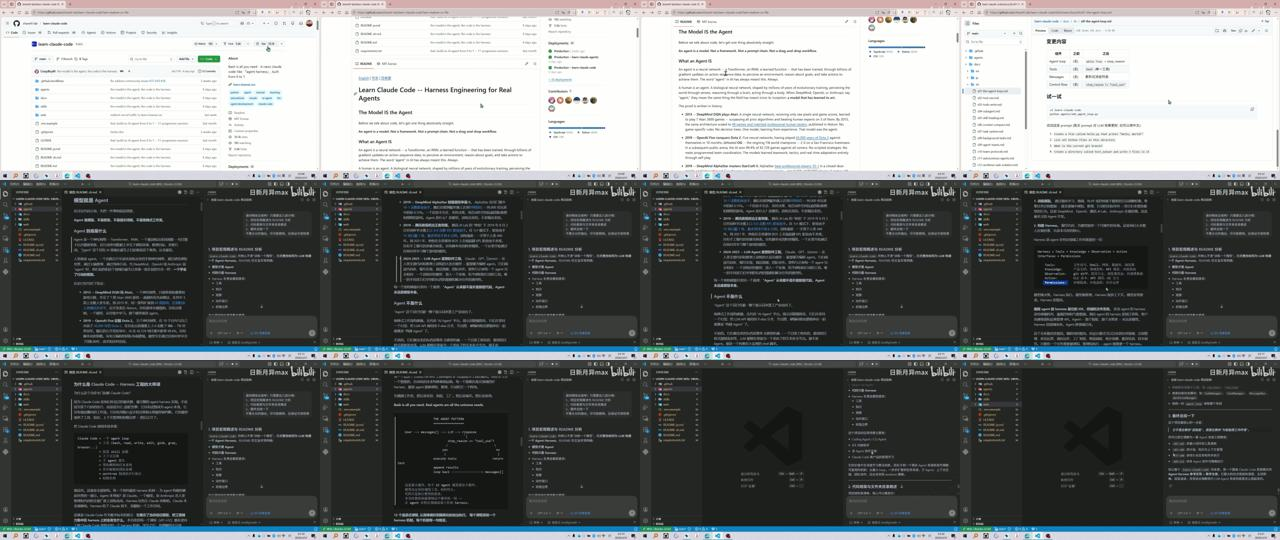
\includegraphics[width=\textwidth]{figures/current-overview-montage.jpg}
\caption{当前 runtime 的 overview montage}
\end{subfigure}
\hfill
\begin{subfigure}[t]{0.48\textwidth}
\centering
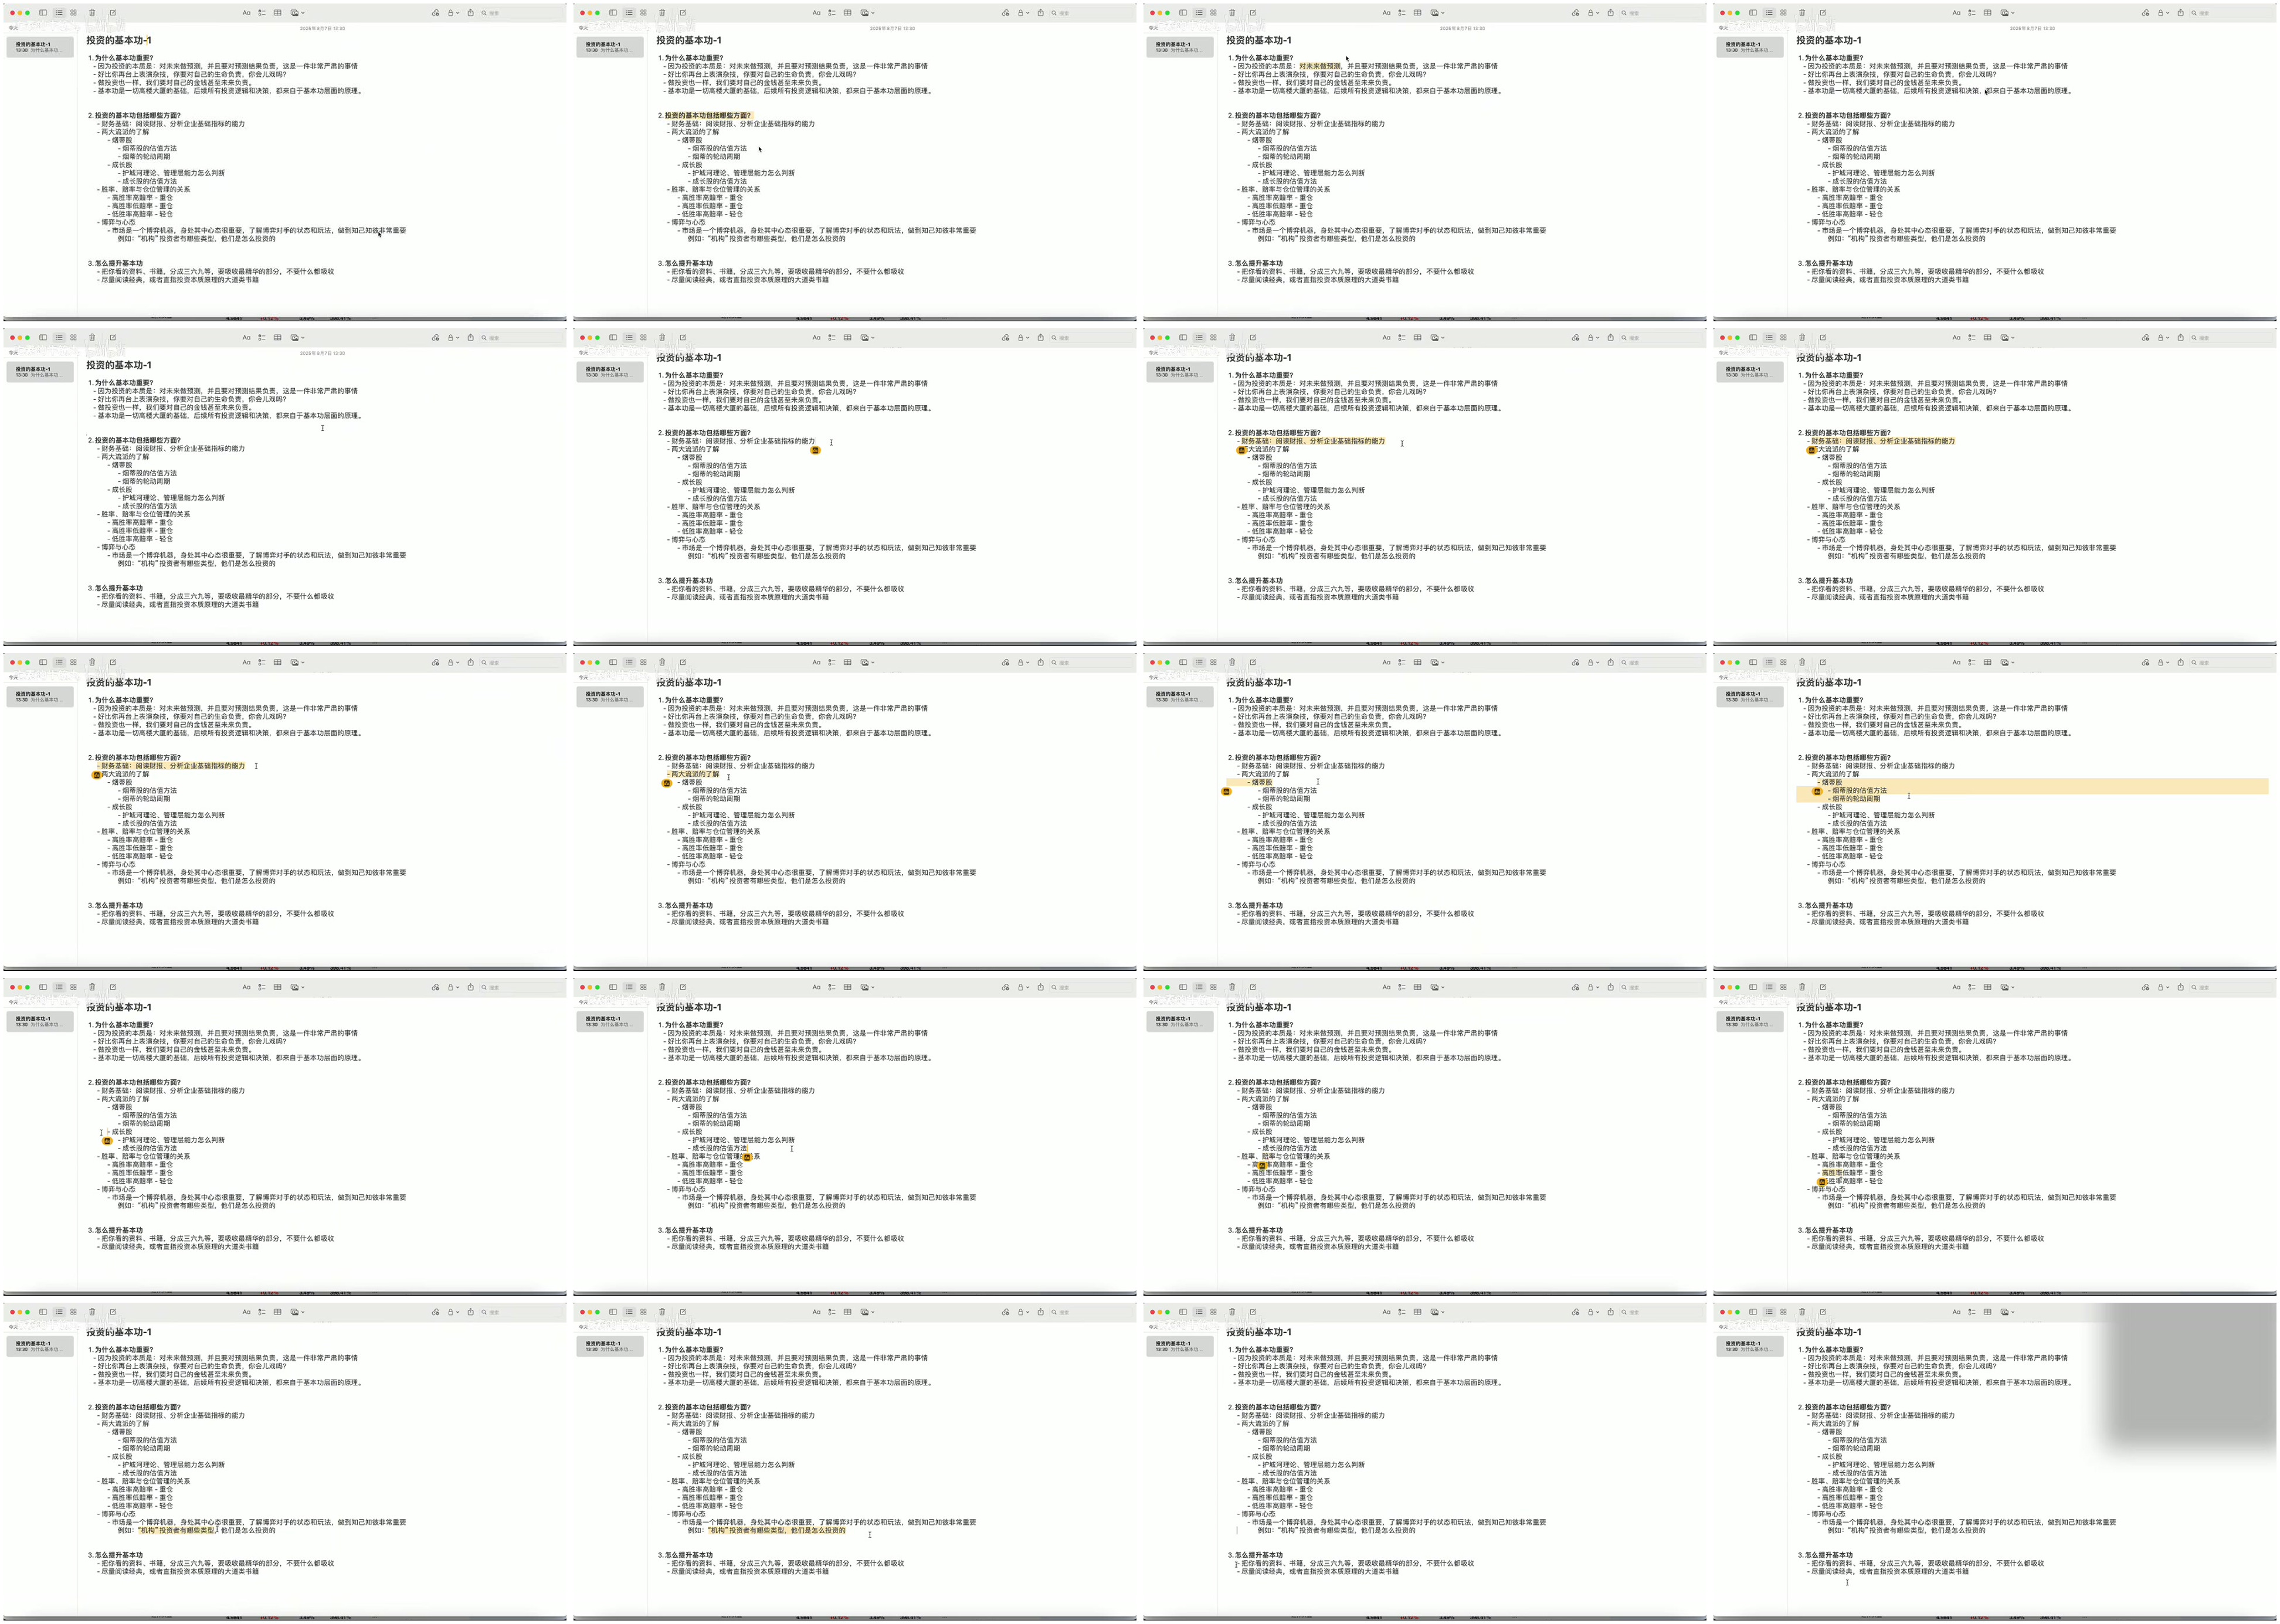
\includegraphics[width=\textwidth]{figures/static-outline-overview.jpg}
\caption{真实 case 中能快速识别单页 outline 的 montage}
\end{subfigure}
\caption{当前 overview 能帮助粗判断视频类型，但还不是“可直接进 PDF 的 figure workflow”。左图来自 runtime 的统一抽样产物；右图来自 \texttt{BV1cptBzFE5Q} case，已经足以驱动策略切换。}
\end{figure}

\small 来源：左图本地路径 \path{/home/fanghaotian/Desktop/src/video-note-pipeline/reports/2026-03-25-apply-review-bv1g5aazheh3/figures/overview-montage.jpg}；右图本地路径 \path{/home/fanghaotian/Desktop/src/video-note-pipeline/.local/workspaces/video-notes/BV1cptBzFE5Q/contacts/overview_montage.jpg}。\normalsize

\subsection{案例证据一：\texttt{static-outline} 视频应尽早切换策略}

\texttt{BV1cptBzFE5Q} 的 retrospective 证明了一个关键点：overview montage 一旦已经显示“画布几乎不变、靠同一页大纲高亮推进”，后续就不该继续走“按章节密集抽大量候选图”的默认路线。真正有效的路径是：

\begin{itemize}
\item 保留一张完整大纲页；
\item 只抽少量高价值裁剪图；
\item 用 TikZ 和结构化重写承担解释任务；
\item 对 provenance 使用图下内嵌小号来源说明，而不是 \texttt{figure + footnotetext}。
\end{itemize}

\begin{figure}[H]
\centering
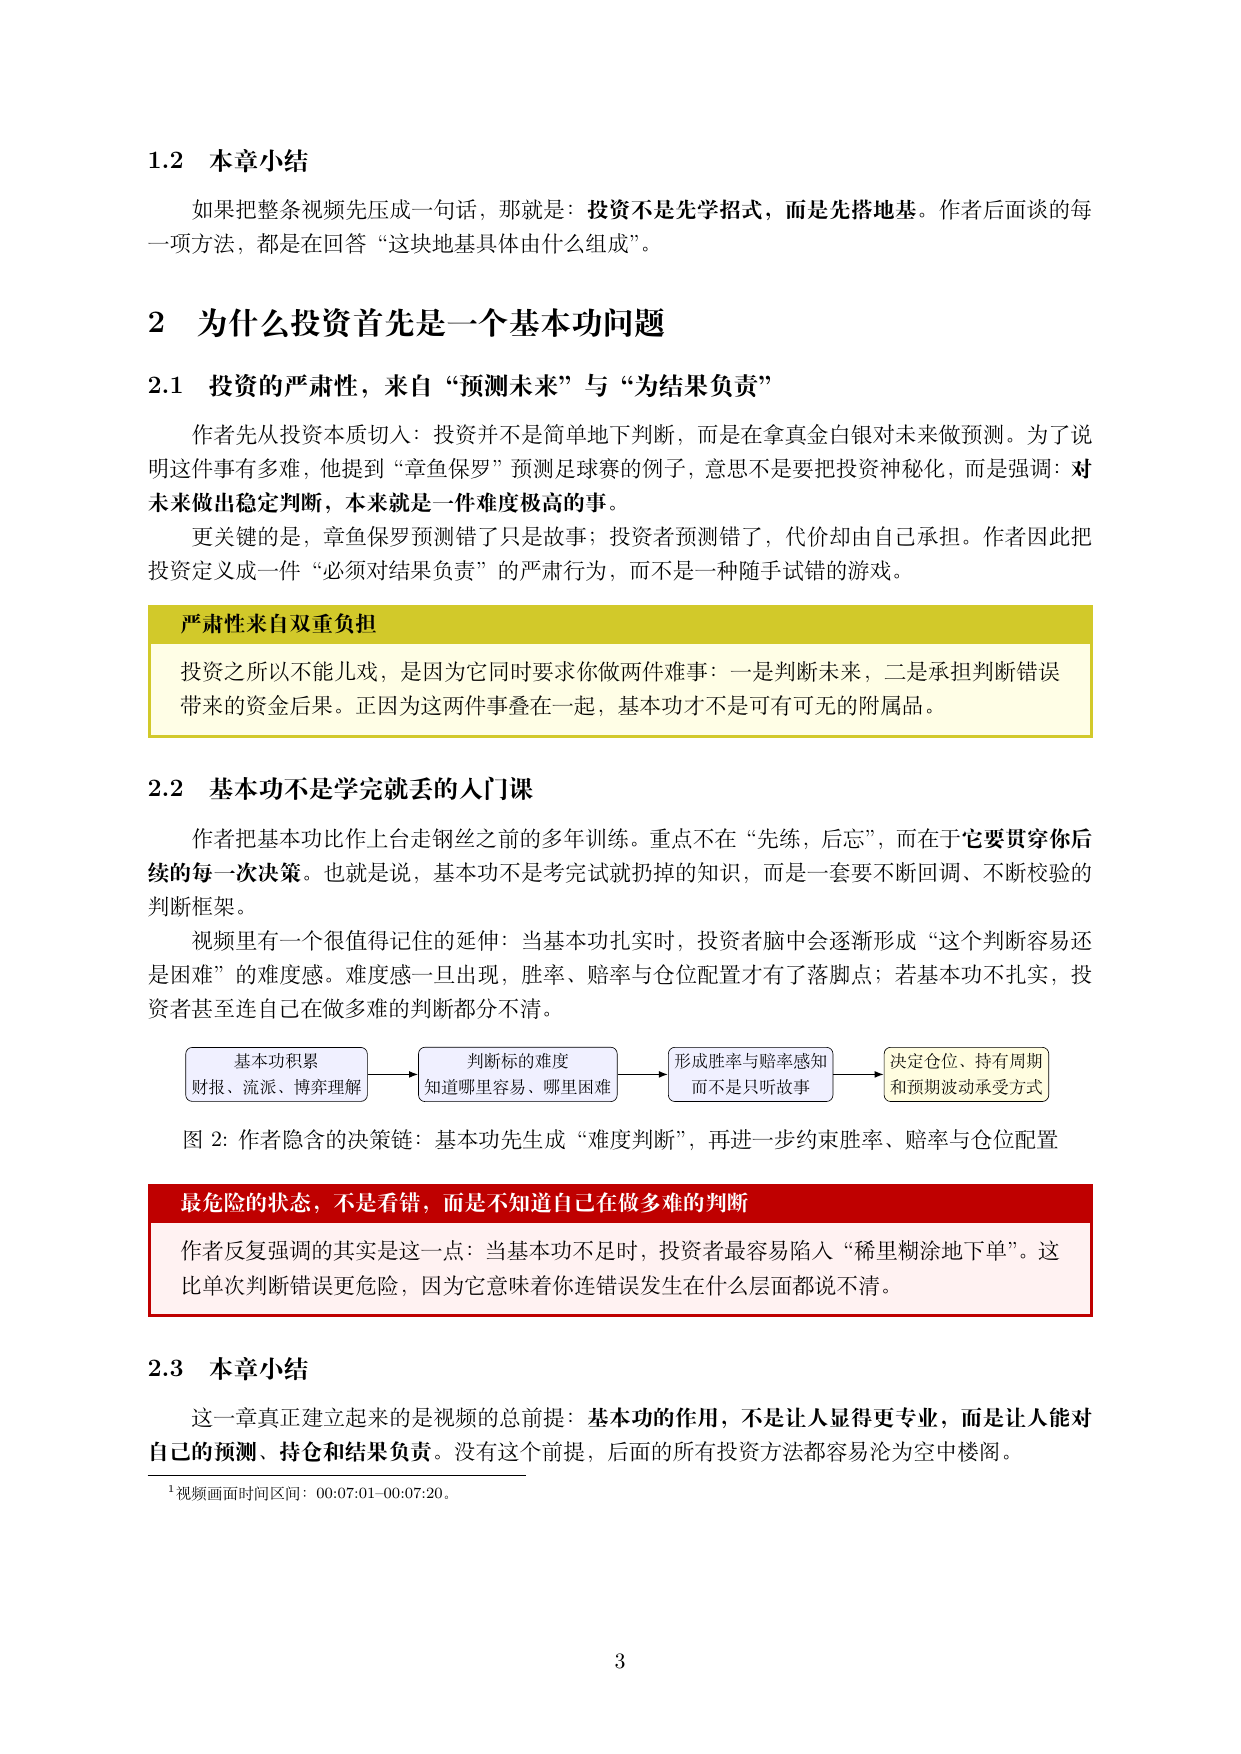
\includegraphics[width=0.74\textwidth]{figures/static-outline-page.png}
\caption{\texttt{static-outline} case 的最终 PDF 页面，说明“少量裁剪图 + 结构化重绘 + 图下 provenance”是可行的稳定交付模式}
\end{figure}

\small 来源：本地路径 \path{/home/fanghaotian/Desktop/src/video-note-pipeline/.local/workspaces/video-notes/BV1cptBzFE5Q/pdf_preview/page-04.png}。页面底部已使用内嵌来源文字，而非漂移风险更高的 \texttt{\textbackslash footnotetext}。\normalsize

\subsection{案例证据二：\texttt{board-heavy} 长视频最需要分层抽帧，而不是逐张回源精抓}

\texttt{BV1tj6wBDEXF} 的 retrospective 和其 \texttt{frame\_manifest.json} 表明，长 AV1 白板 / Excalidraw 视频里，真正高 ROI 的工作流是：

\begin{enumerate}
\item 先以较粗粒度产出大批候选图；
\item 用 montage 快速看完整个候选空间；
\item 候选图足够清晰时，直接 crop candidate；
\item 只有当候选图读不清时，才回到源视频做精确 seek。
\end{enumerate}

这说明“图像工具不够”不是主问题。真正缺的是 runtime 是否内建了 tiered extraction，以及是否有 \texttt{frame\_manifest.json} 记录每张最终图的来源、时间区间、crop 参数和用途。

\subsection{案例证据三：\texttt{commentary} 视频里 OCR 可能几乎完全失效}

\texttt{BV1VaQrBPEg9} 的 retrospective 记录了 403 张候选帧 OCR 全零的事实。这意味着：

\begin{itemize}
\item 对这种视频，继续扩大抽帧和 OCR 只会放大噪声；
\item 最终高价值“图”通常不是视频截图，而是后补的表格、对比图、结构图；
\item 因此 mode routing 必须有 \texttt{commentary / analysis} 分支，而不是强行套到 lecture / tutorial 的截图思路里。
\end{itemize}

\begin{evidencebox}{从三个 case 能归纳出的稳定结论}
\begin{itemize}
\item 不同视频类型需要完全不同的 figure strategy，不能只靠统一抽帧频率。
\item OCR 应该是 probe，而不是默认主流程。
\item 真正稳定的成果来自“图文规划 + 选帧中间层 + provenance”，而不是额外多抽几十张图。
\end{itemize}
\end{evidencebox}

\section{外部方案调研：每个环节有哪些成熟方案}

\subsection{关键帧定位与视频切分}

\subsubsection{FFmpeg：最便宜、最稳的底座}

FFmpeg 官方滤镜文档已经覆盖了当前链路最需要的几个底层能力：

\begin{itemize}
\item \texttt{fps=}：按固定频率抽帧；
\item \texttt{thumbnail}：从一段帧里选代表帧；
\item \texttt{cropdetect}：寻找黑边或稳定裁切边界；
\item \texttt{select='gt(scene, x)'}：依据 scene score 做基础切分。
\end{itemize}

这意味着 P0 阶段并不缺基础工具。\textbf{缺的是把这些滤镜组织成分层策略。}对于当前项目，FFmpeg 足够承担：

\begin{itemize}
\item overview 抽样；
\item 指定时间窗内的 dense candidate extraction；
\item 对黑边、letterbox、固定边栏的初步裁切；
\item 仅在必要时回源视频重抓高分辨率最终图。
\end{itemize}

\subsubsection{PySceneDetect：适合把 transcript window 进一步切细}

\href{https://www.scenedetect.com/docs/latest/api/detectors.html}{PySceneDetect 官方文档}提供了 \texttt{ContentDetector}、\texttt{AdaptiveDetector}、\texttt{ThresholdDetector} 等检测器。它的价值不是“代替字幕对齐”，而是补上字幕没有描述的视觉切换点，例如：

\begin{itemize}
\item PPT 页切换；
\item 屏幕录制中的明显界面变化；
\item 镜头切换；
\item 大纲页中的焦点区域跃迁。
\end{itemize}

我建议把它放在“teaching window 之后、dense candidates 之前”，让 agent 不是盲目在整个字幕段均匀抽样，而是只在真正发生视觉变化的局部区间提高采样密度。

\subsubsection{TransNetV2：适合做强镜头边界，不适合单独承担教学图定位}

\href{https://github.com/soCzech/TransNetV2/blob/master/README.md}{TransNetV2 官方仓库}提供了学习型 shot transition detection。它对电影、综艺、公开视频中的镜头边界很有价值，但对你们当前最重要的三类 case 有局限：

\begin{itemize}
\item \texttt{static-outline}：整页几乎不切镜头，真正重要的是局部高亮变化；
\item \texttt{board-heavy}：白板是渐进累积，重要的是“最终完整状态”，不是 shot boundary；
\item \texttt{commentary}：就算切镜头，也不代表对应知识图。
\end{itemize}

因此 TransNetV2 更适合作为可选增强，而不是第一优先级投入。

\subsubsection{Lecture2Notes：最接近“教学视频里的字幕后可视化链路”}

\href{https://lecture2notes.readthedocs.io/en/latest/end-to-end/frame-extraction.html}{Lecture2Notes 文档}和其 \href{https://lecture2notes.readthedocs.io/en/latest/end-to-end/duplicate-image-removal.html}{duplicate-image-removal 文档}最值得借鉴的地方不在“直接抄实现”，而在流程设计：

\begin{itemize}
\item 先区分 slide frame 与非 slide frame；
\item 对 slide 做黑边裁切、透视矫正；
\item 用图像相似度做重复页去重；
\item 把讲师遮挡、边缘黑框、相机角度等视频噪声当成显式问题来处理。
\end{itemize}

这对你们的启发是：\textbf{crop 不应该只是最后的“手工修一下”，而应成为 figure workflow 的第一等产物。}

\subsubsection{video2slides / YouTube slide extractor：轻量 baseline 的价值}

\href{https://pypi.org/project/video2slides/}{video2slides} 这类项目展示了另一个现实：很多 slide 视频其实可以靠轻量遮罩、边缘剔除、相似度去重、代表帧筛选得到不错结果。它不一定是你们的最终解，但很适合做一个便宜 baseline，用来验证“当前 case 是否值得上更重的 OCR / layout / VLM”。

\begin{table}[H]
\centering
\caption{关键帧定位方案对当前项目的适配性比较}
\begin{tabularx}{\textwidth}{p{2.4cm}p{2.3cm}Yp{2.4cm}}
\toprule
方案 & 主要优势 & 局限 & 对当前项目建议 \\
\midrule
FFmpeg filters & 成本最低、依赖已存在、可直接进 runtime & 语义弱，需要手工组合 & 立即产品化，作为 P0 底座 \\
PySceneDetect & 适合发现字幕之外的视觉变化点 & 仍不理解“教学价值” & P1 接入，做 dense window 辅助 \\
TransNetV2 & 学习型镜头边界更强 & 对单页 outline / 白板增益有限 & P2 评估，不作为首要投入 \\
Lecture2Notes 风格流程 & 最接近教学视频图像管线 & 体系偏重，需选择性借鉴 & 重点借鉴其 crop / dedup / slide filter 思路 \\
video2slides 类工具 & 可做快速 baseline & 对复杂案例天花板低 & 适合做 cheap probe，而非主线路 \\
\bottomrule
\end{tabularx}
\end{table}

\subsection{裁剪、OCR 与版面理解}

\subsubsection{先回答用户的第一个问题：不是“不能 crop”，而是没把 crop 做成产物}

你提出“图片处理工具是不是不够、是不是不能 crop”，从现状看答案是否定的。现有依赖里已经有 Pillow，FFmpeg 也天然支持裁切；本地 case 也已经手工产出了高质量裁剪图。问题在于 runtime 没有下面这些确定性产物：

\begin{itemize}
\item \texttt{crop\_proposal.json}
\item \texttt{full-frame} 与 \texttt{detail-crop} 的并行导出
\item \texttt{frame\_manifest.json} 中的 crop 参数
\item 对 crop 质量的最低检查，如文字可读性、重复度、上下文损失
\end{itemize}

\subsubsection{PaddleOCR：布局和公式页最值得优先借的外部能力}

\href{https://www.paddleocr.ai/latest/en/version3.x/module_usage/layout_analysis.html}{PaddleOCR Layout Analysis} 文档说明其 layout 模块可以给出页面区域结构。对你们最有价值的不是“把整张图 OCR 成文本”，而是：

\begin{itemize}
\item 帮你判断画面里哪里是标题、正文、图示、表格、代码、公式区域；
\item 让 crop 不再只是凭肉眼估；
\item 在 screen demo 和 slide page 里更稳定地切出主要信息区。
\end{itemize}

\href{https://www.paddleocr.ai/main/en/version3.x/module_usage/formula_recognition.html}{公式识别模块} 对数学板书、PPT 公式页尤其重要。它不一定必须上到主流程，但对于公式密集 case，可以作为按需 probe。

\subsubsection{docTR 与 LayoutParser：更适合做可选探针，而不是默认主线}

\href{https://mindee.github.io/doctr/latest/}{docTR} 是 OCR detection + recognition 工具，\href{https://layout-parser.github.io/}{LayoutParser} 则强调布局检测与可组装后处理。二者都适合作为“probe 组件”：

\begin{itemize}
\item 当视频被路由到 \texttt{screen-demo}、\texttt{static-outline}、\texttt{document-heavy} 时启用；
\item 当 OCR 得分、布局稳定性、文本面积超过阈值时再继续；
\item 当进入 \texttt{commentary} 时直接跳过。
\end{itemize}

这比“所有视频一律 OCR”更合理，也更贴合本地 case 证据。

\subsubsection{建议固定四类图，而不是让 agent 每次临场发明}

建议把最终入 PDF 的图固定分成四种：

\begin{enumerate}
\item \texttt{full-frame}：保留完整上下文，例如整页大纲或整张白板。
\item \texttt{detail-crop}：只保留当前段落真正需要看的区域。
\item \texttt{progress-sequence}：当概念是逐步构建时，用一组 2--4 张图表示推进过程。
\item \texttt{synthetic-figure}：当截图本身说不清时，用 TikZ / 表格 / redrawn diagram 承担解释任务。
\end{enumerate}

\begin{findingbox}{关于 crop 的结论}
P0 阶段完全可以只靠 FFmpeg + Pillow + 规则化 crop manifest 获得显著提升；OCR / layout 的收益主要体现在 screen-demo、slide、document-heavy 和 formula-heavy 视频里，应做成按模式启用的 probe。
\end{findingbox}

\subsection{图文规划与中间表示：这是最关键的一层}

\subsubsection{PPT-master 给出的最大启发：先建中间表示，再导出目标文档}

\href{https://raw.githubusercontent.com/hugohe3/ppt-master/main/README.md}{PPT-master README} 最值得借鉴的地方，不是它做的是“文本到 PPT”而不是“视频到 PDF”，而是它明确采用了中间表示思想：先让 AI 输出结构化 SVG / scene，再转换为 PowerPoint 的 DrawingML，从而得到可编辑结果。

你们当前链路最大的问题，正好是少了这一层。现在很容易出现下面的跳跃：

\begin{center}
transcript / overview $\rightarrow$ 直接生成 \texttt{note.tex}
\end{center}

这会导致：

\begin{itemize}
\item 哪一节该放什么图，没有显式约束；
\item 哪张图为什么被选中，没有结构化记录；
\item 章节动机、图的解释职责、外部证据增强都挤在生成正文这一步里；
\item PDF 质量严重依赖 agent 当次发挥。
\end{itemize}

\subsubsection{建议新增的五个中间层}

\begin{table}[H]
\centering
\caption{建议新增的核心 artifact}
{\small
\begin{tabularx}{\textwidth}{p{3.4cm}p{2.6cm}Y}
\toprule
Artifact & 作用 & 最低字段 \\
\midrule
\texttt{outline.json} & 定义章节顺序与动机 & section id, title, objective, source interval \\
\texttt{claims.json} & 把正文拆成可核对的论点单元 & claim id, section id, support type, transcript span, confidence \\
\texttt{figure\_plan.json} & 决定每一节需要什么图以及图承担什么解释职责 & figure id, section id, role, preferred type, source window, must-have / optional \\
\texttt{frame\_manifest.json} & 记录最终图来源与 crop 信息 & figure id, file, source, interval, frame time, crop, purpose \\
\texttt{render\_context.json} & 把上面几层变成 TeX 渲染输入 & metadata, ordered sections, figure refs, callouts, references \\
\bottomrule
\end{tabularx}
}
\end{table}

\subsubsection{推荐的 figure 评分函数}

当一个时间窗里有多张候选图时，建议 runtime 先给出显式分数，agent 再决定是否覆写：

$$
S(f, s) = \alpha R(f) + \beta A(f, s) + \gamma C(f) + \delta N(f) - \lambda D(f)
$$

\begin{itemize}
\item $S(f, s)$：候选帧 $f$ 在当前教学单元 $s$ 下的综合分数
\item $R(f)$：可读性，衡量文字大小、模糊程度、对比度
\item $A(f, s)$：与当前字幕 / 章节窗口的对齐程度
\item $C(f)$：内容完整度，尤其针对 progressive reveal / 白板累积
\item $N(f)$：相对已选图的新增信息量
\item $D(f)$：代价惩罚，例如必须重新 seek 源视频、OCR 失败或 crop 不稳定
\item $\alpha, \beta, \gamma, \delta, \lambda$：根据模式路由设定的权重
\end{itemize}

这个函数不要求一开始就完美，但它会迫使 runtime 把“选图理由”变成显式数据，而不是全靠人的临场直觉。

\subsection{PDF 构建：保留 LaTeX，重构输入层}

\subsubsection{为什么不建议现在就迁移到 Typst 或 Quarto}

\href{https://typst.app/docs/}{Typst 官方文档} 和 \href{https://quarto.org/docs/output-formats/pdf-basics.html}{Quarto PDF 文档} 都说明它们各有优势：

\begin{itemize}
\item Typst 在现代写作体验、模板化、编译速度上更友好；
\item Quarto 在研究报告、Markdown 驱动工作流、表格与数据可视化编排上很强；
\item 但 Quarto 的高质量 PDF 仍依赖 LaTeX 引擎，而你们当前已有的中文模板、TikZ、callout、图片规则都已沉淀在 LaTeX 上。
\end{itemize}

因此当前最合理的路线不是更换 renderer，而是改造输入层：

\begin{itemize}
\item 让 TeX 只负责最后编排；
\item 让叙事规划、figure plan、provenance、外部证据增强在 TeX 之前完成；
\item 把 provenance 的默认写法从 \texttt{figure + footnotetext} 改成图下内嵌来源块。
\end{itemize}

\subsubsection{为什么现有模板里的 provenance 推荐写法应调整}

统一 wrapper 的模板注释目前仍推荐：

\begin{lstlisting}[caption={当前模板注释推荐的 provenance 模式}]
\begin{figure}[H]
\centering
\includegraphics[width=\textwidth]{...}
\caption{... \protect\footnotemark}
\end{figure}
\footnotetext{视频画面时间区间：00:12:31--00:12:46。}
\end{lstlisting}

但本地 \texttt{BV1cptBzFE5Q} case 已经证明，这种写法在接近分页边界时会把来源说明挤到下一页，违背“图和来源留在同页”的要求。建议默认改成：

\begin{lstlisting}[caption={建议的图下内嵌 provenance 模式}]
\begin{figure}[H]
\centering
\includegraphics[width=\textwidth]{figures/fig_xxx.jpg}
\caption{关键图：......}
\end{figure}
{\footnotesize
\noindent 来源：视频 00:12:31--00:12:46，原始候选图 chapter_0031.jpg，
最终使用裁剪参数 840x500+80+20。}
\end{lstlisting}

\begin{findingbox}{关于 PDF 引擎的结论}
短中期不建议切换 Typst / Quarto。对你们当前项目，最大的 PDF 质量提升来自“结构化中间层 + route-specific 模板 + provenance 修正 + PDF QA”，而不是更换排版引擎。
\end{findingbox}

\subsection{联网增强：应该做，但必须模式化}

你提出“构建 PDF 时是否可以上网搜索”这一点，我的判断是：\textbf{可以，而且在某些模式下非常值得；但不要放在最后 build 阶段，也不要对所有视频默认开启。}

\subsubsection{建议的三档联网策略}

\begin{table}[H]
\centering
\caption{联网增强的模式化策略}
\begin{tabularx}{\textwidth}{p{3cm}p{3.1cm}Y}
\toprule
模式 & 是否联网 & 建议行为 \\
\midrule
faithful lecture-note & 默认关闭或仅补拓展阅读 & 保持对讲者叙事的忠实性，不主动纠正文稿主线 \\
commentary / analysis & 建议开启 & 区分视频原话、外部事实、整理者推断；对核心结论做背景补足与事实核验 \\
evidence-sensitive & 必须开启 & 对公共政策、金融、医学等内容优先引用一手来源，并显式记录证据链 \\
\bottomrule
\end{tabularx}
\end{table}

\subsubsection{为什么它不应该发生在 build 阶段}

如果把联网放在 TeX 生成之后，通常只会造成两种坏结果：

\begin{itemize}
\item 找到的信息没有进入章节动机和图文结构，只能被硬塞成附录；
\item 外部事实和视频原叙事被混写，最终失去 provenance。
\end{itemize}

更合理的做法是在 \texttt{claims.json} 定稿前，增加一个可选的 \texttt{evidence\_enrichment.json}：

\begin{itemize}
\item 哪个 claim 需要外部来源；
\item 使用了哪些网页 / PDF / 论文；
\item 是 \texttt{corroborate}、\texttt{correct} 还是 \texttt{background-only}；
\item 证据强弱与冲突情况如何。
\end{itemize}

\section{逐条回答用户的五个问题}

\subsection{1. 图片处理工具是不是不够，不能 crop？}

\textbf{不是。}现有工程已经具备 FFmpeg 与 Pillow，理论上完全能做 crop。真正的短板是缺少围绕 crop 的 workflow 和数据结构。现阶段最有效的升级不是再装一个图像库，而是：

\begin{itemize}
\item 把 crop proposal、crop variant、crop provenance 变成 runtime 产物；
\item 给每张关键图至少保留 \texttt{full-frame} 与 \texttt{detail-crop} 两种版本；
\item 对 screen-demo / slide / formula-heavy 视频再按需启用 OCR / layout probe。
\end{itemize}

\subsection{2. 视频处理是否不够好，导致定位不准？}

\textbf{是，而且这是当前最明显的工程短板。}现有 runtime 的定位本质上还是全片均匀抽样，只适合给 mode 提供初始建议，不适合直接产最终图。最需要增加的是：

\begin{enumerate}
\item 把 transcript 聚成教学单元，而不是逐条 subtitle 处理；
\item 结合 scene change、chapter 边界和语义峰值定位高价值窗口；
\item 在窗口内做 dense candidate extraction；
\item 候选图可读时先 crop candidate，只有必要时回源精抓。
\end{enumerate}

\subsection{3. PDF 构建是否有更好的方式让逻辑更连贯？}

\textbf{有，但关键不是换 PDF 引擎，而是先做中间层。}我建议的核心变化是：不要再从 transcript 直接跳到 \texttt{note.tex}，而是先构建章节动机、论点列表、图的解释职责，再渲染模板。这样生成出来的 PDF 会更接近一份“研究型讲义”，而不是“把口播和截图堆在一起的长文”。

\subsection{4. 构建 PDF 时是否可以联网搜索更多资源？}

\textbf{可以，但要按模式开关。}对讲义型视频，联网更多是补“拓展阅读”；对评论 / 分析型视频，联网可以显著提升文档的背景层与证据质量；对证据敏感主题，甚至应当强制联网。最重要的是把这一步放在 outline / claims 定稿前，并显式分开“视频原话”“外部事实”“整理者推断”。

\subsection{5. 历史 case 是否应该进一步利用？}

\textbf{应该，而且应该直接变成评测集。}你们已经有足够典型的 case：

\begin{itemize}
\item \texttt{BV1cptBzFE5Q}: \texttt{static-outline}
\item \texttt{BV1tj6wBDEXF}: \texttt{board-heavy}
\item \texttt{BV1VaQrBPEg9}: \texttt{commentary}
\item \texttt{bv1z9qzbgewv}: \texttt{visual-light}
\end{itemize}

下一步不应该只是“再做几次漂亮案例”，而是把这些 case 变成回归测试与 PDF QA 集。

\section{建议的目标架构}

\subsection{总体设计：从字幕到 PDF 的六层链路}

\begin{figure}[H]
\centering
\resizebox{\textwidth}{!}{
\begin{tikzpicture}[
    node distance=0.8cm and 0.7cm,
    box/.style={draw, rounded corners, align=center, minimum height=1cm, minimum width=2.5cm, fill=blue!4},
    decision/.style={draw, diamond, aspect=2, align=center, fill=yellow!12},
    arrow/.style={-Latex, thick}
]
\node[box] (transcript) {Transcript\\Subtitle / ASR};
\node[box, right=of transcript] (outline) {Outline / Claims\\教学单元与论点};
\node[decision, right=of outline] (route) {Mode Routing\\视频类型分支};
\node[box, right=of route] (figureplan) {Figure Plan\\图的职责规划};
\node[box, below=of figureplan] (windows) {Teaching Windows\\候选时间窗};
\node[box, left=of windows] (candidates) {Dense Candidates\\高召回候选帧};
\node[box, left=of candidates] (manifest) {Frame Manifest\\crop / provenance};
\node[box, below=of candidates] (render) {Render Context\\章节-图-来源组合};
\node[box, right=of render] (tex) {TeX Renderer\\模板 + TikZ + 图};
\node[box, right=of tex] (qa) {PDF QA\\版面与来源检查};

\draw[arrow] (transcript) -- (outline);
\draw[arrow] (outline) -- (route);
\draw[arrow] (route) -- (figureplan);
\draw[arrow] (figureplan) -- (windows);
\draw[arrow] (windows) -- (candidates);
\draw[arrow] (candidates) -- (manifest);
\draw[arrow] (manifest) -- (render);
\draw[arrow] (render) -- (tex);
\draw[arrow] (tex) -- (qa);
\draw[arrow] (outline.south) |- (render.north);
\end{tikzpicture}
}
\caption{建议的目标架构：在字幕与 TeX 之间加入结构化中间层，避免“直接从 transcript 跳成 PDF”}
\end{figure}

\subsection{建议扩展的模式分类}

当前 wrapper 只有 \texttt{talking-head}、\texttt{visual-light}、\texttt{static-outline}、\texttt{board-heavy} 四类。我建议至少补成六类：

\begin{table}[H]
\centering
\caption{建议的 mode taxonomy}
{\small
\begin{tabularx}{\textwidth}{p{2.7cm}p{2.9cm}Y}
\toprule
Mode & 典型视觉特征 & 推荐图像策略 \\
\midrule
\texttt{talking-head} & 人像主导，视觉内容稀薄 & 少量 representative frames，更多依赖结构化写作与自制图 \\
\texttt{visual-light} & 偶尔有关键 slide / product UI & overview 后做定向时间窗抽帧，保留少量关键图 \\
\texttt{static-outline} & 单页大纲、文字密、变化慢 & 整页锚点图 + 少量 detail-crop + TikZ，总体少截图 \\
\texttt{board-heavy} & 白板、手写、渐进累积 & 高召回候选图，优先最终完整态，必要时补中间步骤序列 \\
\texttt{screen-demo} & 软件界面、操作步骤、局部控件频繁变化 & scene change + OCR/layout probe + detail-crop / sequence \\
\texttt{commentary} & 画面只承担陪衬，价值在论证结构 & 少量代表帧 + 表格 / TikZ / 外部证据增强 \\
\bottomrule
\end{tabularx}
}
\end{table}

\subsection{针对每种模式的 figure workflow}

\subsubsection{\texttt{static-outline}}

\begin{itemize}
\item 先通过 overview 确认“单画布 + 高亮推进”。
\item 生成完整大纲页的高分辨率锚点图。
\item 每章最多只保留 0--1 张 detail-crop。
\item 优先用 TikZ、表格、总结框承担解释。
\end{itemize}

\subsubsection{\texttt{board-heavy}}

\begin{itemize}
\item 先在高价值窗口做 dense candidates。
\item montage 后优先找“最终完整可读状态”。
\item 候选图足够清晰时直接 crop-first。
\item 只在文字或公式读不清时回源视频精抓。
\end{itemize}

\subsubsection{\texttt{screen-demo}}

\begin{itemize}
\item 把字幕单元与 scene change 结合，切到真正操作步骤窗口。
\item 用 OCR / layout 估计可交互控件和主要信息区。
\item 每个关键操作步骤导出 \texttt{full-screen} 与 \texttt{detail-crop}。
\item 对连续操作用 2--4 张 progress sequence，而不是截满整段视频。
\end{itemize}

\subsubsection{\texttt{commentary / analysis}}

\begin{itemize}
\item 把截图数量控制在最小必要集。
\item 重点投入在 outline、claim graph、对比表、因果链图。
\item 如有必要，开启联网背景增强。
\item 严格区分视频观点、外部事实和整理者推断。
\end{itemize}

\subsection{推荐的目录树与 artifact 合约}

\begin{lstlisting}[caption={建议固定的 case 目录树}]
case/
  assets/
  cover.jpg
  transcript.srt
  transcript.json
  outline.json
  claims.json
  figure_plan.json
  frame_manifest.json
  render_context.json
  evidence_enrichment.json   # optional
  figures/
    final/
    candidates/
    crops/
  montages/
  previews/
  note.tex
  note.pdf
  build.log
\end{lstlisting}

\begin{riskbox}{artifact 管理原则}
\begin{itemize}
\item \texttt{final}、\texttt{evidence}、\texttt{scratch} 必须分层。
\item 编译垃圾不应和最终交付混在一起。
\item 如果一次 run 做过后续精修，应保留 append-only run ledger，而不是只留下最终目录态。
\end{itemize}
\end{riskbox}

\subsection{PDF QA：不要再停在“编过就算”}

建议把 PDF QA 固定成四类检查：

\begin{enumerate}
\item \textbf{结构检查}：章节顺序、目录、图文引用、总结章节是否完整。
\item \textbf{图像检查}：是否模糊、是否重复、是否裁掉关键信息、是否误抓动画过渡帧。
\item \textbf{provenance 检查}：每张视频图是否附具体时间区间，同页呈现是否稳定。
\item \textbf{版面检查}：跨页漂移、caption 溢出、公式截断、表格过窄、预览页抽检。
\end{enumerate}

\section{实施路线：按 ROI 排序}

\subsection{P0：先补最值钱的中间层}

\begin{itemize}
\item 在 runtime 中新增 \texttt{capture\_keyframes}：
  teaching windows $\rightarrow$ dense candidates $\rightarrow$ montage $\rightarrow$ crop-first $\rightarrow$ frame manifest
\item 新增 \texttt{figure\_plan.json} 与 \texttt{frame\_manifest.json}
\item 将 provenance 默认写法改成图下内嵌来源块
\item 在 mode routing 中加入 \texttt{screen-demo} 与 \texttt{commentary / analysis}
\end{itemize}

\subsection{P1：引入 probe 型视觉增强}

\begin{itemize}
\item 接入 PySceneDetect，把字幕窗口进一步细分
\item 接入 PaddleOCR layout analysis，专门服务于 slide / UI / document-heavy 画面
\item 对公式密集 case 增加 formula probe
\item 建立 crop quality / readability 的自动阈值
\end{itemize}

\subsection{P2：引入更强的语义规划}

\begin{itemize}
\item 让 agent / VLM 参与 \texttt{figure\_plan.json} 的生成与覆写
\item 引入 \texttt{evidence\_enrichment.json}，按模式启用联网背景核验
\item 用更显式的 claim graph 支撑正文结构与图的放置
\end{itemize}

\subsection{P3：评估更远期替代方案}

\begin{itemize}
\item 评估 TransNetV2 对 screen-demo / mixed-media 视频是否带来实质收益
\item 小规模验证 Typst / Quarto 作为未来报告型模式的备选 renderer
\item 仅当 LaTeX 模板演进成本成为瓶颈时，再考虑 renderer 迁移
\end{itemize}

\section{评测集与验收指标}

\subsection{建议先固化四个 benchmark case}

\begin{itemize}
\item \texttt{BV1cptBzFE5Q}：\texttt{static-outline}
\item \texttt{BV1tj6wBDEXF}：\texttt{board-heavy}
\item \texttt{BV1VaQrBPEg9}：\texttt{commentary / analysis}
\item \texttt{bv1z9qzbgewv}：\texttt{visual-light}
\end{itemize}

\begin{figure}[H]
\centering
\begin{subfigure}[t]{0.48\textwidth}
\centering

\includegraphics[width=\textwidth]{figures/video-triptych.jpg}
\caption{最终整理出的代表帧组合图}
\end{subfigure}
\hfill
\begin{subfigure}[t]{0.48\textwidth}
\centering
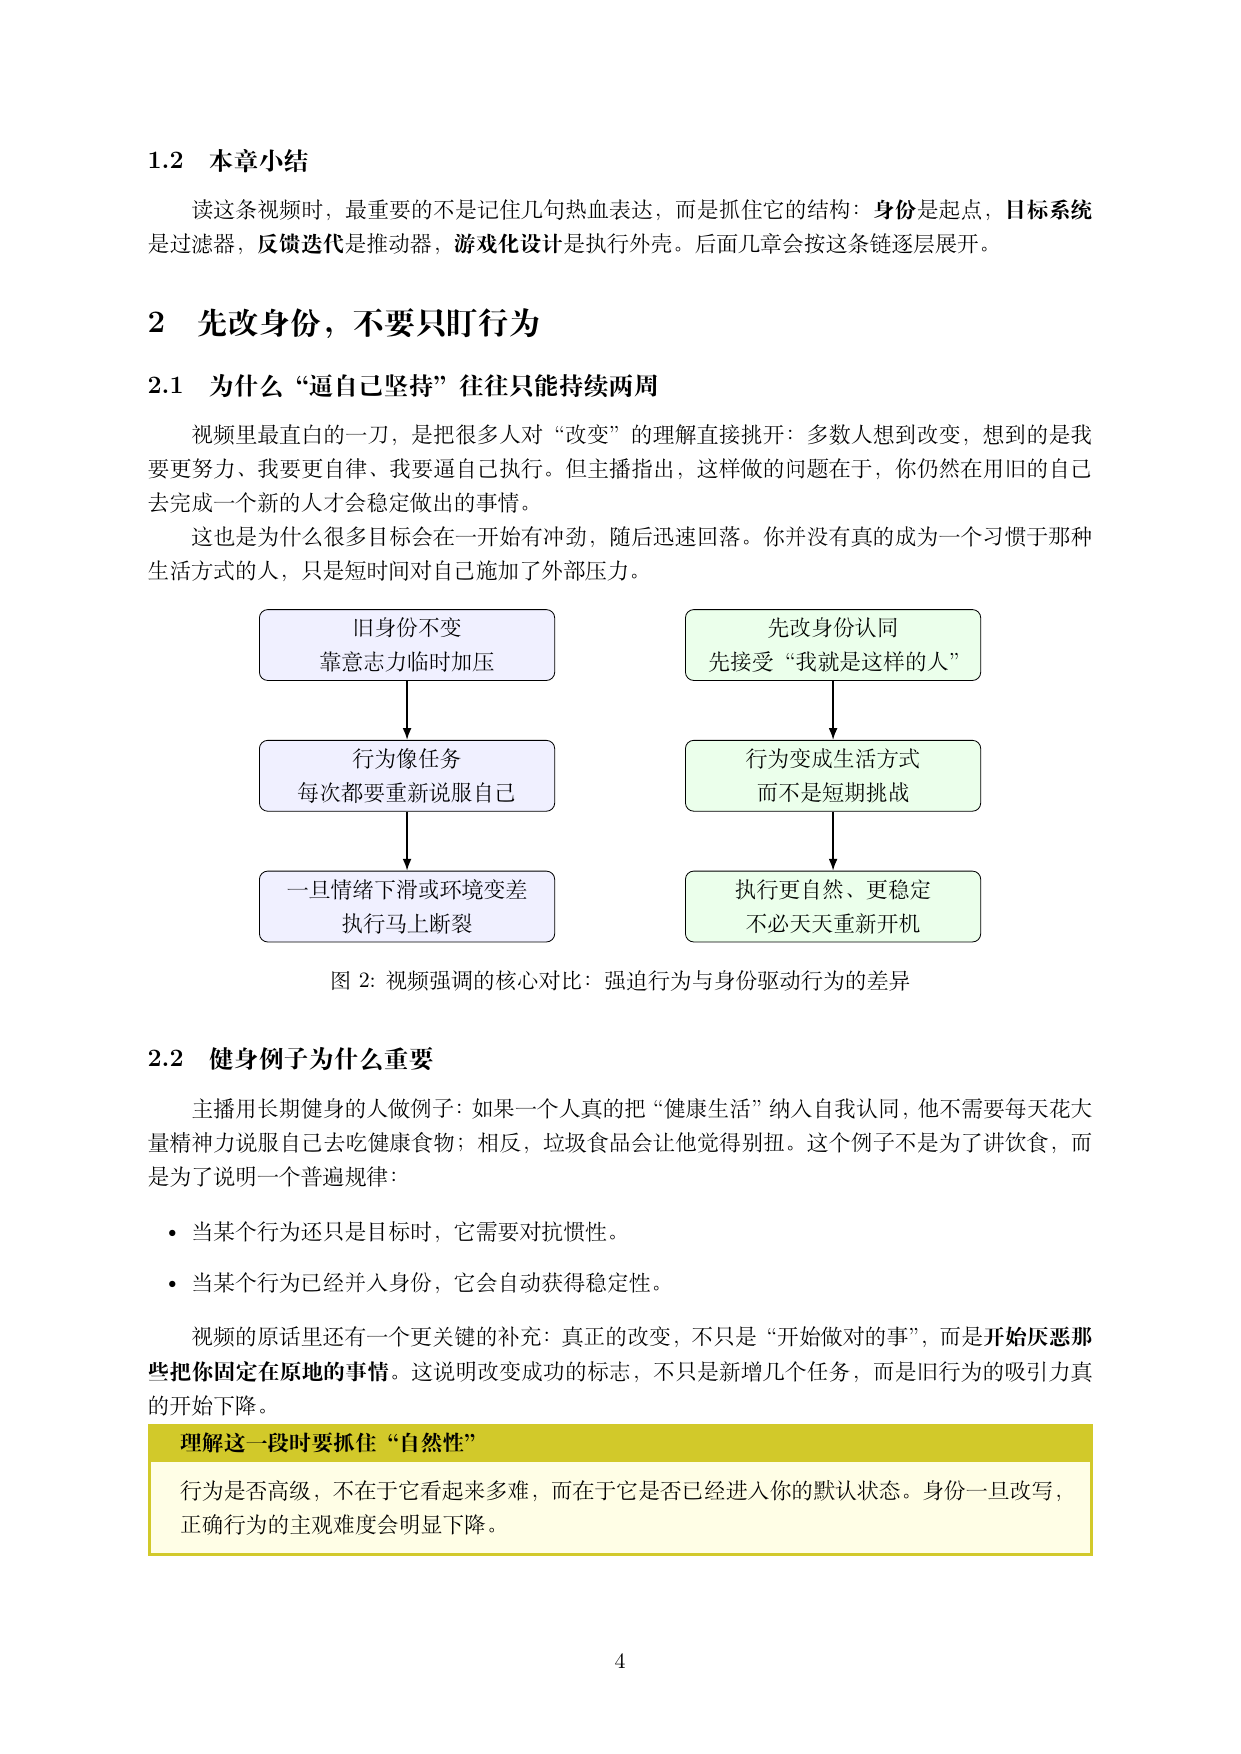
\includegraphics[width=\textwidth]{figures/final-page-example.png}
\caption{最终 PDF 页面示例}
\end{subfigure}
\caption{本地现有 case 已经证明，只要 figure workflow 与图文规划到位，最终 PDF 可以明显好于原始 overview 抽样阶段}
\end{figure}

\small 来源：左图 \path{/home/fanghaotian/Desktop/src/video-note-pipeline/.local/workspaces/video-notes/bv1z9qzbgewv/figures/video_triptych.jpg}；右图 \path{/home/fanghaotian/Desktop/src/video-note-pipeline/.local/workspaces/video-notes/bv1z9qzbgewv/pdf_preview/page-05.png}。\normalsize

\subsection{不要只测“能否出 PDF”}

建议的核心指标包括：

\begin{table}[H]
\centering
\caption{建议的验收指标}
\begin{tabularx}{\textwidth}{p{3cm}Yp{2.5cm}}
\toprule
指标 & 解释 & 类型 \\
\midrule
Figure Readability & 图中文字、公式、控件是否清晰可读 & 硬指标 + 人审 \\
Figure Novelty & 最终图之间是否大量重复 & 自动 + 人审 \\
Figure Alignment & 图是否真对应正文讨论的教学单元 & 人审主导 \\
Provenance Completeness & 每张视频图是否有时间区间、来源和 crop 记录 & 自动可检 \\
Narrative Coherence & 章节动机、图和正文是否相互支撑 & 人审主导 \\
PDF Layout Stability & 是否存在脚注漂移、图片裁切、页边溢出 & 自动预览 + 人审 \\
Build Reproducibility & 是否能在当前机器稳定复现产物 & 自动可检 \\
\bottomrule
\end{tabularx}
\end{table}

\subsection{建议的最小回归测试}

\begin{itemize}
\item 结构测试：确保 \texttt{outline.json}、\texttt{claims.json}、\texttt{figure\_plan.json}、\texttt{frame\_manifest.json} 字段齐全
\item 渲染测试：确保所有 figures 路径可解析，\texttt{note.tex} 可编译
\item QA 测试：自动导出预览页，对重复图和缺失 provenance 做规则检查
\item 回归测试：四个 benchmark case 的页数、图数量、核心图类型维持在合理范围内
\end{itemize}

\section{风险、边界与不建议做的事}

\subsection{不要在没有中间层之前盲目上重型视觉模型}

如果现在直接接入一堆 OCR、VLM、布局模型，但没有固定 artifact，很容易出现：

\begin{itemize}
\item 生成一堆额外 JSON，却不知道哪一层该消费；
\item 同一张图被不同模块重复判断，结果互相冲突；
\item agent prompt 更长，真实稳定性反而下降。
\end{itemize}

\subsection{不要把 OCR 当作所有视频的默认解}

本地 \texttt{commentary} case 已经证明 OCR 可以完全无效。OCR 应该是 probe，不是默认主干。

\subsection{不要让联网增强改写“忠实讲义”的基本契约}

对于教学视频，联网带来的背景补足很有价值，但不能悄悄把讲者的主张改写成整理者自己的文章。外部来源必须明确标注其角色。

\subsection{不要把最好的 case 误当成“流程天然稳定产物”}

你们已有的好案例里，有不少质量来自后续人工 refinement。如果未来要把这些能力真正下沉到 runtime，就必须保留 append-only run ledger，并把“这一步是自动稳定完成的”与“这一步是后期人工补救的”分开记录。

\section{结论与后续问题}

\subsection{已经有充分证据支持的结论}

\begin{itemize}
\item 当前问题的主轴不是“缺少图像工具”，而是“缺少字幕之后的结构化中间层”。
\item 最值钱的升级是 figure workflow 产品化：teaching windows、dense candidates、crop-first、frame manifest、render context。
\item mode routing 至少应补 \texttt{screen-demo} 与 \texttt{commentary / analysis} 两类。
\item LaTeX 不是眼下的瓶颈；应优先修结构化输入与 provenance，而不是迁移 renderer。
\item 历史 case 已足以构成 benchmark / eval 套件。
\end{itemize}

\subsection{大概率正确但仍值得继续验证的推断}

\begin{itemize}
\item PySceneDetect 会在 screen-demo 和 mixed-media 视频上带来明显收益，但在 \texttt{static-outline} 和 \texttt{board-heavy} 上收益可能有限。
\item PaddleOCR layout / formula probe 对公式页、PPT 页、界面录屏会有明显价值，但对 commentary 价值不高。
\item VLM 适合作为 \texttt{figure\_plan} 的覆写器，而不适合直接替代确定性 frame workflow。
\end{itemize}

\subsection{下一步最值得做的三件事}

\begin{enumerate}
\item 在 \texttt{video-note-pipeline} 里实现 P0 版关键帧捕获层，核心产物为 \texttt{capture\_keyframes}、\texttt{figure\_plan.json} 与 \texttt{frame\_manifest.json}。
\item 修正模板默认 provenance，并把 PDF QA 固定成流程的一部分。
\item 把四个典型 case 收敛成回归评测集，用来验证 mode routing 和 figure workflow 是否真正变稳定。
\end{enumerate}

\appendix

\section{来源清单}
\small
\begin{longtable}{p{1.5cm}p{1.7cm}p{4.0cm}p{6.8cm}}
\toprule
Source ID & 模态 & 标题 / 标签 & 链接或路径 \\
\midrule
\endfirsthead
\toprule
Source ID & 模态 & 标题 / 标签 & 链接或路径 \\
\midrule
\endhead
L1 & Local & 旧 \texttt{bilibili-render-pdf} 规则 & \path{/home/fanghaotian/.codex/skills/video-note-skill/skills/bilibili-render-pdf/SKILL.md} \\
L2 & Local & 统一 wrapper 模板注释 & \path{/home/fanghaotian/Desktop/src/agent-basic-skill/skills/video-note-render-pdf/assets/notes-template.tex} \\
L3 & Local & \texttt{overview.py} & \path{/home/fanghaotian/Desktop/src/video-note-pipeline/src/video_note_pipeline/frames/overview.py} \\
L4 & Local & \texttt{commands.py} 中 \texttt{overview\_case} & \path{/home/fanghaotian/Desktop/src/video-note-pipeline/src/video_note_pipeline/commands.py} \\
L5 & Local & \texttt{pyproject.toml} & \path{/home/fanghaotian/Desktop/src/video-note-pipeline/pyproject.toml} \\
L6 & Local & \texttt{mode-routing.md} & \path{/home/fanghaotian/Desktop/src/agent-basic-skill/skills/video-note-render-pdf/references/mode-routing.md} \\
L7 & Local & \texttt{BV1cptBzFE5Q} retrospective & \path{/home/fanghaotian/Desktop/src/video_notes/evlove/WORKFLOW_RETROSPECTIVE_BV1cptBzFE5Q_2026-03-25.md} \\
L8 & Local & \texttt{BV1tj6wBDEXF} retrospective & \path{/home/fanghaotian/Desktop/src/video_notes/evlove/WORKFLOW_RETROSPECTIVE_BV1tj6wBDEXF_2026-03-25.md} \\
L9 & Local & \texttt{BV1VaQrBPEg9} retrospective & \path{/home/fanghaotian/Desktop/src/video_notes/evlove/WORKFLOW_RETROSPECTIVE_BV1VaQrBPEg9_2026-03-25.md} \\
L10 & Local & \texttt{frame\_manifest.json} 示例 & \path{/home/fanghaotian/Desktop/src/video-note-pipeline/.local/workspaces/video-notes/BV1tj6wBDEXF/frame_manifest.json} \\
L11 & Local & 总复盘 & \path{/home/fanghaotian/Desktop/src/video_notes/evlove/WORKFLOW_RETROSPECTIVE_2026-03-25.md} \\
W1 & Web & FFmpeg Filters Documentation & \url{https://ffmpeg.org/ffmpeg-filters.html} \\
W2 & Web & PySceneDetect Documentation & \url{https://www.scenedetect.com/docs/latest/api/detectors.html} \\
W3 & Web & TransNetV2 GitHub README & \url{https://github.com/soCzech/TransNetV2/blob/master/README.md} \\
W4 & Web & Lecture2Notes duplicate image removal & \url{https://lecture2notes.readthedocs.io/en/latest/end-to-end/duplicate-image-removal.html} \\
W5 & Web & Lecture2Notes frame extraction & \url{https://lecture2notes.readthedocs.io/en/latest/end-to-end/frame-extraction.html} \\
W6 & Web & video2slides PyPI & \url{https://pypi.org/project/video2slides/} \\
W7 & Web & PaddleOCR Layout Analysis & \url{https://www.paddleocr.ai/latest/en/version3.x/module_usage/layout_analysis.html} \\
W8 & Web & PaddleOCR Formula Recognition & \url{https://www.paddleocr.ai/main/en/version3.x/module_usage/formula_recognition.html} \\
W9 & Web & docTR Documentation & \url{https://mindee.github.io/doctr/latest/} \\
W10 & Web & LayoutParser & \url{https://layout-parser.github.io/} \\
W11 & Web & PPT-master README & \url{https://raw.githubusercontent.com/hugohe3/ppt-master/main/README.md} \\
W12 & Web & Quarto PDF Basics & \url{https://quarto.org/docs/output-formats/pdf-basics.html} \\
W13 & Web & Typst Documentation & \url{https://typst.app/docs/} \\
W14 & Web & Docling Documentation & \url{https://docling-project.github.io/docling/} \\
\bottomrule
\end{longtable}
\normalsize

\section{一个可直接执行的最小技术任务单}

\begin{enumerate}
\item 在 runtime 新增 \texttt{capture\_keyframes.py}，输入 \texttt{transcript.json + outline.json + mode}，输出 \texttt{candidates/}、\texttt{montages/}、\texttt{frame\_manifest.json}。
\item 新增 \texttt{figure\_plan.json}，每节至少给出图类型、解释职责、时间窗与 must-have 标记。
\item 把 LaTeX 模板里的 provenance 默认模式改成图下内嵌来源块。
\item 新增 \texttt{commentary} 与 \texttt{screen-demo} 路由，并为其分别定义 figure strategy。
\item 将 \texttt{BV1cptBzFE5Q}、\texttt{BV1tj6wBDEXF}、\texttt{BV1VaQrBPEg9}、\texttt{bv1z9qzbgewv} 固化为 benchmark case。
\end{enumerate}

\end{document}
